

\begin{table*}[t!]
% \renewcommand\arraystretch{1.2}
\centering
\caption{Mamba vs. Transformer on D4RL datasets.}
\label{Mamba vs Transformer}
\resizebox{1.0\textwidth}{!}{
\begin{tabular}{l| l  | r r r |rrr|rrr}
\toprule
\specialrule{0em}{1.5pt}{1.5pt}
\toprule
\multicolumn{2}{c|}{Environment} & \multicolumn{3}{c|}{HalfCheetah} & \multicolumn{3}{c|}{Hopper} & \multicolumn{3}{c}{Walker2d} \\
\toprule
 \multicolumn{2}{c|}{Dataset} & Med-Expert & Medium & Med-Replay & Med-Expert & Medium & Med-Replay & Med-Expert & Medium & Med-Replay  \\
\midrule[1pt]
\multirow{2}{*}{Effectiveness} & Transformer & \textbf{94.21\scriptsize{$\pm$ 0.46}} & \textbf{42.28\scriptsize{$\pm$ 1.18}}  & \textbf{41.28\scriptsize{$\pm$ 0.21}} & 108.32\scriptsize{$\pm$ 0.95} & 72.58\scriptsize{$\pm$ 0.54} & \textbf{91.32\scriptsize{$\pm$ 0.66}} & \textbf{111.36\scriptsize{$\pm$ 0.46}} & \textbf{85.96 \scriptsize{$\pm$ 0.46}} & \textbf{89.21\scriptsize{$\pm$ 1.42}}\\
& Mamba & 92.21\scriptsize{$\pm$ 0.60} & 41.92\scriptsize{$\pm$ 0.11} & 39.68\scriptsize{$\pm$ 0.13} & \textbf{110.82\scriptsize{$\pm$ 0.56}} & \textbf{73.65\scriptsize{$\pm$ 1.23}} & 82.65\scriptsize{$\pm$ 1.15} & 108.31\scriptsize{$\pm$ 0.52} & 78.26\scriptsize{$\pm$ 0.55} & 70.92\scriptsize{$\pm$ 1.21}\\
\toprule
\multirow{2}{*}{Efficiency (hour)} & Transformer & \multicolumn{3}{c|}{37.10\scriptsize{$\pm$ 0.22}}  & \multicolumn{3}{c|}{22.23\scriptsize{$\pm$ 0.15}} & \multicolumn{3}{c}{33.77\scriptsize{$\pm$ 0.26}}\\
& Mamba & \multicolumn{3}{c|}{\textbf{28.56\scriptsize{$\pm$ 0.18}}}  & \multicolumn{3}{c|}{\textbf{18.15\scriptsize{$\pm$ 0.16}}} & \multicolumn{3}{c}{\textbf{26.25\scriptsize{$\pm$ 0.21}}}\\
\bottomrule
\specialrule{0em}{1.5pt}{1.5pt}
\bottomrule
\end{tabular}
}
\vspace{-0.4cm}
\end{table*}


% \multirow{2}{c|}{performance}

\section{Method}

% \setlength{\belowcaptionskip}{-0.2cm} %调整图片标题与下文距离 
% \setlength{\abovecaptionskip}{-0.0cm} %调整图片标题与图距离

In this section, we first compare Mamba and transformer models in the D4RL dataset, and investigate the potential of Mamba in RL tasks. Then, We present DM-H, which can handle long-term dependencies from contexts with high effectiveness and efficiency, as shown in Figure~\ref{DM-H}.

\subsection{Mamba vs. Transformer in RL tasks}

We first consider the Algorithm Distillation (AD) as the baseline, which is a classic in-context RL method using a transformer as the backbone \cite{8}. 
AD can predict high-quality actions by recalling the historical trajectories from the context, but it also incurs higher computational costs.
Under the same settings, we replace the transformer in the AD algorithm with Mamba to compare their effectiveness and efficiency. 
% AD trains the model with across-episodic contexts, where the size of the context is equal to 4 times the length of the trajectory. Since the context covers multiple trajectories, the model can predict better actions by recalling the historical experience, but it also induces higher computational costs.

As shown in Table~\ref{Mamba vs Transformer}, the simple backbone replacement did not significantly improve effectiveness. Regarding efficiency, Mamba brings predictable improvements, thus saving training time under the same settings. Compared with the attention mechanism acting on state pairs, Mamba uses a data-dependent selection mechanism acting on each state independently, which brings a more efficient method of recalling long-term memory. However, since states in RL tasks commonly exhibit sequential relationships, the attention mechanism is more suitable for capturing the information between states, thereby outperforming Mamba in terms of effectiveness.
To this end, we aim at a new in-context RL approach that leverages Mamba's strengths in processing long-term memory while preserving high-quality predictions from transformers.

\begin{figure*}
    \centering
    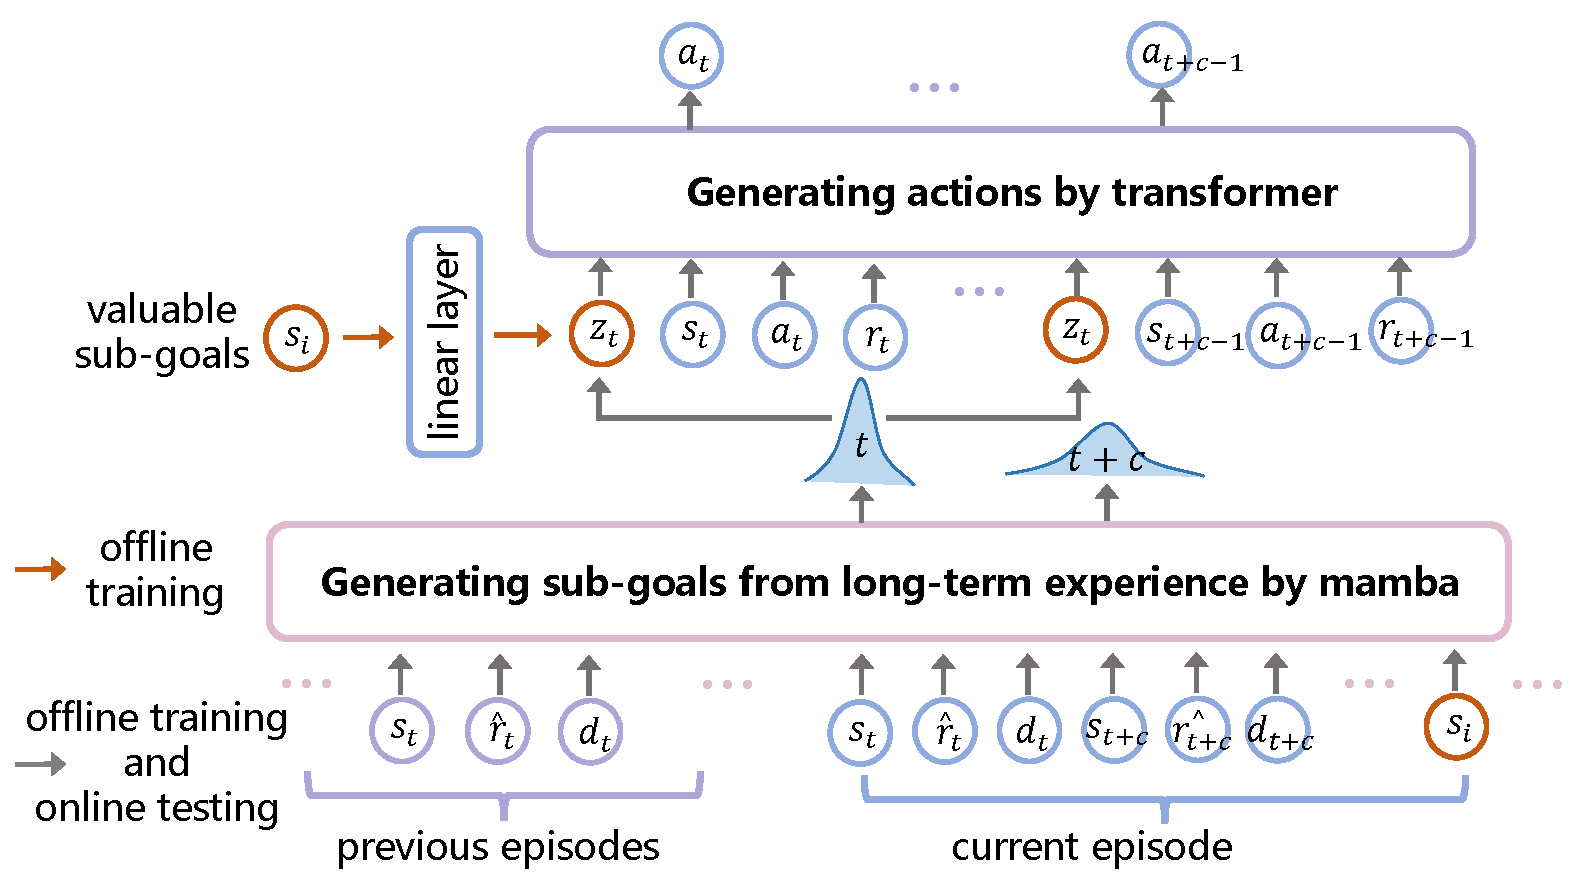
\includegraphics[width=0.9\columnwidth]{Results/HM.pdf}
    \caption{The architecture of DM-H. During offline training, Mamba module generates sub-goals from long-term experience, where the long-term experience consists of multiple historical trajectories arranged in ascending order of the total rewards. Based on the generated sub-goals, the transformer is required to predict better actions by supervising the expert behaviors. Meanwhile, the linear layer feeds the valuable sub-goals into the transformer module and associates them with the generated actions. During online testing, DM-H can automatically improve its performance in a trial-and-error manner without requiring gradient updates.
    }
    \label{DM-H}
\end{figure*}

\subsection{Decision Mamba-Hybrid}

In-context RL can automatically improve its performance through trial-and-error when across-episodic contexts serve as prompt conditions. Specifically, an across-episodic context consisting of $n$ trajectories is represented as $(\tau^{1},\tau^{2},\dots,\tau^{n})$, where
\begin{equation}
    \tau^{i}= (s_0^i,a_0^i,r_0^i,d_0^i,\dots,s_T^i,a_T^i,r_T^i,d_T^i).
\label{coe}
\end{equation}
The trajectories are sorted according to their total rewards, i.e.,$\sum_{t=0}^T{r_t^1}\leq\sum_{t=0}^T{r_t^2}\leq\dots\leq\sum_{t=0}^T{r_t^n}$. With autoregressive training and generation, the transformer can uncover meaningful patterns from multiple trajectories and improve itself conditioned on experience. However, the quadratic complexity of the attention mechanism suffers from huge computational costs along with the growth in task horizon. Inspired by Mamba's success with long sequences, we propose that Mamba handles across-episodic contexts and preserves local short-term sequences for the transformer. For Mamba, we reconstruct the long-term sequences $(\tau_m^{1},\tau_m^{2},\dots,\tau_m^{n})$ from across-episodic contexts. Each $\tau_m^{i}$ is denoted as
\begin{equation}
\tau_m^{i}=(s_0^i,\hat{r}_0^i,d_0^i,s_{c}^i,\hat{r}_{c}^i,d_{c}^i,\dots,s_{kc}^i,\hat{r}_{kc}^i,d_{kc}^i),
\label{mamba}
\end{equation}
where $c$ represents the local sequence length for the transformer, $T-c\leq kc \leq T$, and $\hat{r}_c^i=\sum_{t=c}^{2c-1}{r_t^i}$ is the sum of $c$ steps rewards. Mamba module will generate sub-goals to prompt the transformer, where the sub-goal is represented by a vector $\textbf{z}$ sampled from a multivariate Gaussian distribution. Then, the local short-term sequence is represented as:
\begin{equation}
\tau_\textbf{z}^{i,j}=(\textbf{z}_j^i,s_j^i,a_j^i,r_j^i, \textbf{z}_{j}^i,s_{j+1}^i,a_{j+1}^i,r_{j+1}^i, \dots,\textbf{z}_{j}^i,s_{j+c-1}^i,a_{j+c-1}^i,r_{j+c-1}^i),
\label{transformer}
\end{equation}
where $\tau_\textbf{z}^{i,j}$ starts from the generation step $j\in\{0,c,\dots,kc\}$ and completes $c$ steps actions based on the generated sub-goal $\textbf{z}_j^i$.

\subsection{Decision Mamba-Hybrid with Valuable Sub-goals}

DM-H links Mamba and the transformer through the sub-goal $\textbf{z}$ to efficiently recall long-term contexts while ensuring high-quality predictions. As sub-goals are commonly hidden in the offline data, Mamba must infer them along with the transformer training. However, it remains to be seen whether the transformer will benefit from $\textbf{z}$ or ignore it and only imitate expert behaviors based on the local context. Therefore, we select extra high-value states from the offline data and transform them into sub-goals $\textbf{z}$ to align actions generated by the transformer.

\noindent\textbf{Valuable sub-goals.}~~
Intuitively, a sub-goal should be highly valuable for the agent to reach and have a high probability of appearing at subsequent time steps of the current state in the trajectory. When reached sequentially, these states should mark milestones in the trajectory, making it highly probable that the agent successfully performs the task. In this point, the valuable sub-goals guide the agent through the task, meaning they have the same purpose as the returns-to-go in the Decision Transformer \cite{2}. Therefore, we can model this behavior by finding states with high accumulated reward values in the trajectory. Specifically, for state $s_i$ at timestep $i$, the value of state $s_j$ at timestep $j$ is $\sum_{t=i+1}^jr_k$, where $i+1\leq j\leq T$. However, this may prioritize the last state of trajectories when the environment only provides positive rewards. To encourage selecting states that are close to the current state $s_i$, we divide the accumulated rewards by the distance between their timesteps $\sum_{t=i+1}^jr_k/(j-i)$. With the punishment of the distance, the weighted average of accumulated rewards can identify the short-term and important future states.

% \noindent\textbf{HM with Valuable Sub-goals.}~~
Based on the selected sub-goals, we reconstruct the local short-term sequence (Equation~\eqref{transformer}) by replacing $\textbf{z}$ generated from Mamba. The reconstructed local short-term sequence is represented as:
\begin{equation}
\tau_g^{i,j}=(f(s_g^i),s_j^i,a_j^i,r_j^i, f(s_g^i),s_{j+1}^i,a_{j+1}^i,r_{j+1}^i, \dots,f(s_g^i),s_{j+c-1}^i,a_{j+c-1}^i,r_{j+c-1}^i),
\label{g_transformer}
\end{equation}
where $s_g^i$ is the most valuable sub-goal for state $s_j^i$ and $f$ is a linear layer that maps $s_g^i$ to the same dimension of $\textbf{z}_{j}^i$. The reconstructed local short-term sequence aligns the actions generated by the transformer with subsequent high-valued states. Since Equation~\eqref{transformer} is consistent with the reconstructed sequence except for $\textbf{z}_{j}^i$, this encourages Mamba module to generate high-value sub-goals from the long-term context to ensure that the transformer module predicts similar actions.

\subsection{Implementation of DM-H}

\noindent\textbf{Architecture.}~~
We feed $n$ trajectories into Mamba module, which results in $3\times n\times T/c$ tokens, with one token for each of the three modalities: state, reward, and completion. In the transformer module, we feed $4\times c$ tokens, with one token for each of the four modalities: sub-goal, state, action, and reward. To create the token embeddings, we train a linear layer for each modality, which transforms the raw inputs into the desired embedding dimension, followed by layer normalization \cite{26}. Finally, we freeze a linear layer that maps the high-value sub-goals $s_g$ in Equation~\eqref{g_transformer} to the same dimensions as the sub-goals $\textbf{z}$ generated by Mamba.

\noindent\textbf{Offline Training and Online Testing.}~~
During offline training, we are given a dataset of offline trajectories, where the trajectories can be suboptimal.
In each iteration, we sample minibatches of trajectories from the dataset. 
Then, Mamba module first predicts the sub-goals $\textbf{z}_t$ every $c$ steps, given the input token $s_t$ and past trajectories. Then, the transformer module autoregressively predicts $c$ steps of actions $\{a_t,\dots,a_{t+c-1}\}$ given $\textbf{z}_t$ and $\{s_t,\dots,s_{t+c-1}\}$. 
Meanwhile, we use the weighted average of accumulated rewards to select valuable sub-goals from the offline data and feed them to the transformer model to predict the same $c$ steps actions.
The predicted actions are evaluated with either cross-entropy loss or mean-squared error, depending on whether the actions are discrete or continuous. The losses from each step are averaged and updated in all modules end-to-end. At online testing, we roll out the DM-H with multiple trajectories and report the return of the last trajectory. Following the configuration from related works \cite{1,8}, we set a context size across $n=4$ episodes.
The pseudocode for DM-H is summarized in Appendix~\ref{appendix A}. Source code and more hyperparameters are described in Appendix~\ref{appendix B}.

